% !TEX encoding = UTF-8
% !TEX TS-program = pdflatex
% !TEX root = ../tesi.tex

%**************************************************************
\chapter{Metodologia di sviluppo}
\label{cap:metodologia-lavoro}
%**************************************************************

\intro{In questo capitolo viene descritta la metodologia di lavoro e i ruoli adottati dal \textit{team} di sviluppo.}\\

%**************************************************************
\section{Scrum}
\href{https://www.scrum.org/about}{\textit{Scrum}} è un \textit{framework} \textit{agile} per lo sviluppo, consegna e manutenzione di prodotti \textit{software} e non.
\textit{Scrum} è progettato per l'utilizzo in \textit{team} di dimensione ridotta. 
Di seguito vengono descritti ruoli, fasi e artefatti del \textit{framework}.

\subsection{Ruoli}

\subsubsection{Scrum Master}
Lo \textit{Scrum Master} aiuta il \textit{team} di sviluppo ad apprendere e applicare \textit{Scrum} per conseguire valore di \textit{business}. Lo \textit{Scrum Master} fa tutto ciò che è in suo potere per aiutare il \textit{team}, il \textit{Product Owner} e l'organizzazione ad avere successo. \textit{Scrum Master} non è il \textit{manager} dei membri del \textit{team}, né è un \textit{project manager}, \textit{team} \textit{leader}, o rappresentante del \textit{team}.
Lo scopo dello \textit{Scrum Master} è:
\begin{itemize}
    \item aiutare a rimuovere gli ostacoli durante lo sviluppo;
    \item evitare interferenze esterne;
    \item aiutare il \textit{team} ad adottare al meglio le pratiche di sviluppo \textit{agile};
    \item fare in modo che tutti applichino \textit{Scrum} nel miglior modo possibile.
\end{itemize}

\subsubsection{Product Owner}
Il \textit{Product Owner} ha la responsabilità di massimizzare il ritorno sugli investimenti (ROI), di identificare le caratteristiche del prodotto, traducendole in una lista di priorità, di decidere cosa dovrebbe andare in cima alla lista per il prossimo \textit{Sprint}, e di riassegnare le priorità, aggiornandole con continuità. Il \textit{Product Owner} detiene la responsabilità di profitto del prodotto, se questo è commerciale. In \textit{agile} il \textit{Product Owner} rappresenta il cliente e nell'applicazione di \textit{Scrum} può e deve:
\begin{itemize}
    \item definire il \textit{Product Backlog}, le \textit{user stories} e gli \textit{acceptance criteria};
    \item definire le priorità nel \textit{Product Backlog} e la data di rilascio del prodotto;
    \item accettare o rifiutare quanto sviluppato;
    \item cancellare lo \textit{Sprint} se risulta fallimentare o poco utile.
\end{itemize}


\subsubsection{Team di sviluppo}
Il \textit{team} di sviluppo è composto da un insieme di persone, in genere meno di dieci, e si occupa di sviluppare quanto definito dal \textit{Product Owner}. Il \textit{team} \textit{Scrum} deve essere \textit{"cross-funzionale"}, ovvero includere tutte le competenze necessarie allo sviluppo del prodotto. I membri del \textit{team} devono essere proattivi e aperti allo studio di tecnologie che vanno oltre le loro competenze.
Il \textit{team} di sviluppo:
\begin{itemize}
    \item costruisce il prodotto definito dal \textit{Product Owner};
    \item possiede tutte le conoscenze per ottenere un prodotto potenzialmente rilasciabile alla fine di ogni \textit{Sprint};
    \item è auto organizzato, con un alto grado di autonomia e responsabilità;
    \item decide quanti e quali elementi del \textit{Product Backlog} sviluppare;
    \item ha la responsabilità di sviluppo, \textit{test} e rilascio del prodotto;
    \item non possiede un \textit{team} \textit{leader}, in quanto in \textit{Scrum} nel \textit{team} di sviluppo sono considerati tutti di pari livello.
\end{itemize}

Nel corso dello stage i ruoli erano così suddivisi:
\begin{itemize}
    \item \textit{scrum master}: Bledar Gogaj
    \item \textit{team} di sviluppo: Alessandro Discalzi, Tania Parolin
    \item \textit{product owner}: Marco Lionello
\end{itemize}

\subsection{Artefatti}

\subsubsection{Product Backlog}
Il \textit{Product Backlog} è un elenco di funzionalità, centrate sul cliente e ordinato per priorità, esiste e si evolve per tutta la durata del prodotto. Il \textit{Product Backlog} definisce quindi tutto ciò che deve essere fatto ed include una moltitudine di voci, più nello specifico:
\begin{itemize}
    \item nuove funzionalità da implementare;
    \item obbiettivi di miglioramento;
    \item lavori di ricerca;
    \item difetti da risolvere, se in numero contenuto;
\end{itemize}
Un buon \textit{Product Backlog} è \textit{\textbf{DEEP}}:
\begin{itemize}
    \item \textbf{dettagliato}, con maggior attenzione alle voci di priorità più alta;
    \item \textbf{stimato}: per ogni voce deve esserci una stima per il completamento, la stima viene definita dal \textit{team} di sviluppo;
    \item \textbf{emergente}: il \textit{Product Backlog} viene aggiornato in base alla variabilità del progetto;
    \item \textbf{prioritizzato}: le voci sono ordinate per priorità, quelle con priorità più alta forniscono maggior valore al prodotto.
\end{itemize}
Nel corso del progetto di stage per gestire il \textit{Product Backlog} è stato utilizzato \textit{\href{https://taiga.io/}{Taiga}}, un tool per la gestione di progetti \textit{agile}.
\begin{figure}[h]
    \begin{center}
    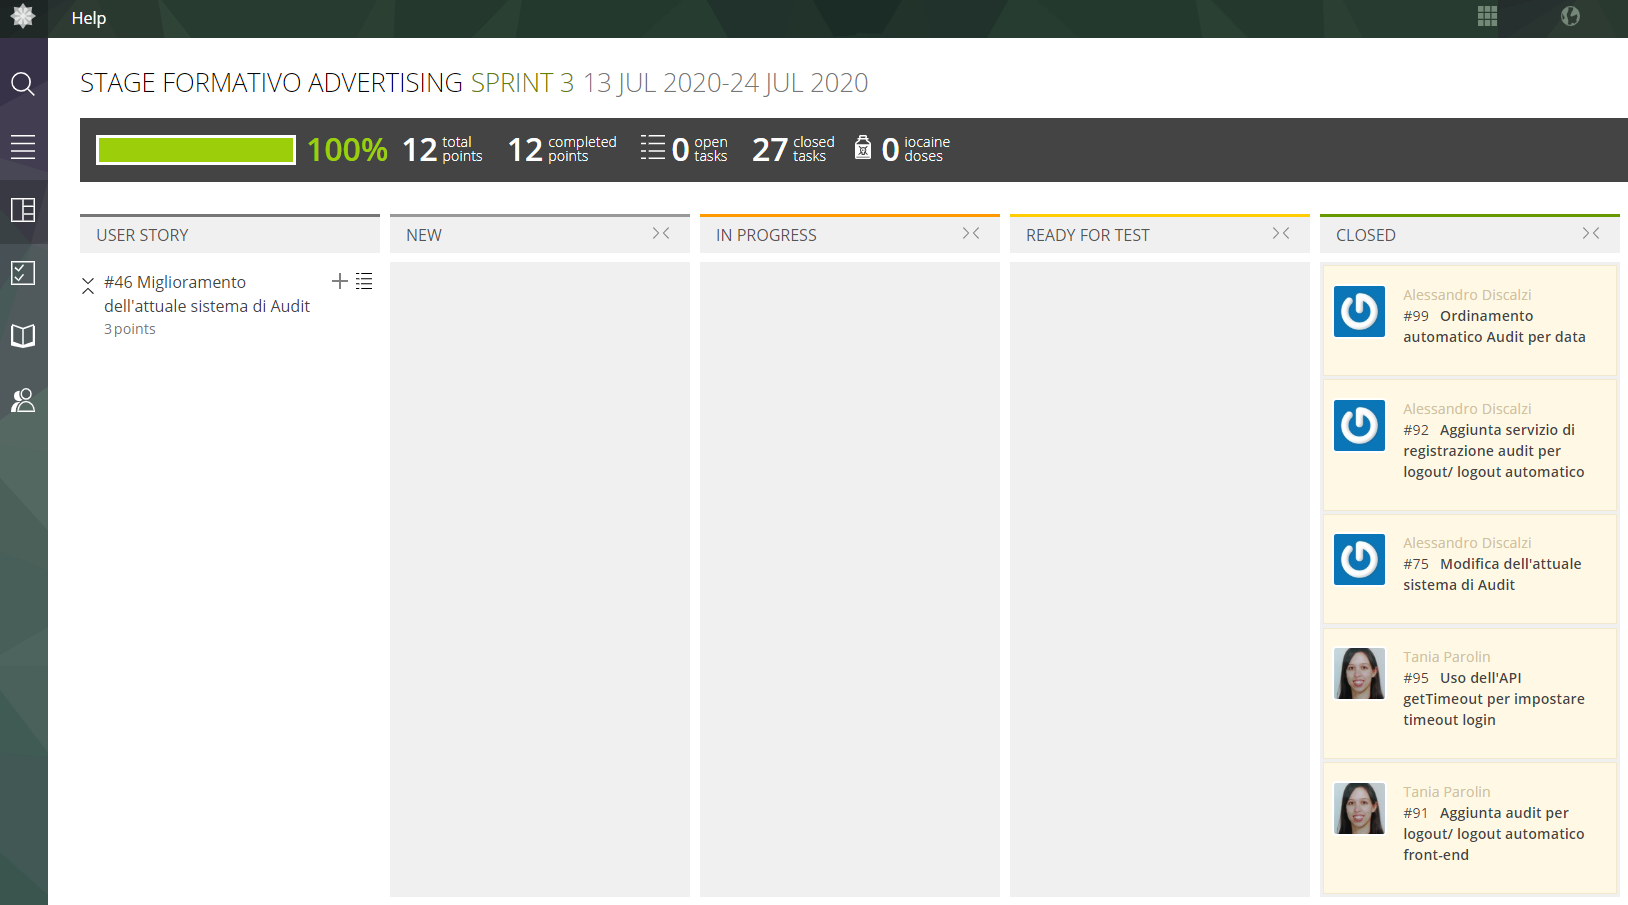
\includegraphics[width=1.2\textwidth]{taiga}
    \caption{Screenshot del backlog presente su Taiga rispetto uno degli \textit{Sprint} terminati}
    \label{fig:figure14}
    \end{center}
\end{figure}
\\Nel \textit{Product Backlog} di AMS la lista delle attività eseguite, in ordine di priorità, è la seguente:
\begin{itemize}
    \item \textit{design} e realizzazione della base di dati;
    \item \textit{design} e realizzazione del template di base per i contenuti pubblicitari;
    \item realizzazione della funzione di \textit{preview} di un contenuto;   
    \item gestione autenticazione e autorizzazione in base ai ruoli;
    \item realizzazione dei servizi di \textit{back-end}; 
    \item \textit{design} e implementazione della \gls{ui}\glsfirstoccur{};
    \item integrazione \textit{front-end} e \textit{back-end};
    \item implementazione della creazione di nuovi contenuti;
    \item implementazione della modifica di un contenuto;
    \item miglioramento \gls{ux}\glsfirstoccur{} e \gls{ui};
    \item inizio stesura documentazione;
    \item implementazione sistema di \textit{auditing};
    \item miglioramento dei contenuti di esempio;
    \item predisposizione di \textit{Oracle};
    \item implementazione \textit{breadcrumbs};
    \item aggiunta controlli di validazione;
    \item completamento della documentazione;
    \item controlli sull'accessibilità del \textit{software};
    \item miglioramento pipeline di \gls{ci}\glsfirstoccur{};
    \item predisposizione demo.
\end{itemize}

\subsubsection{Definition of done}
Durante ogni \textit{Sprint} ciò che viene fatto costituisce un prodotto potenzialmente rilasciabile, questo deve essere approvato dal \textit{Product Owner}, dallo \textit{Scrum Master} e dal \textit{team} di sviluppo prima dell'inizio dello \textit{Sprint} successivo. La \textit{definition of done} è un insieme di regole che definiscono quando ciò che viene fatto può essere definito rilasciabile.
La \textit{definition of done} adottata durante lo stage è la seguente:
\begin{itemize}
    \item AMS (Advertising Management System) deve essere stato compilato senza \textit{warning};
    \item il \textit{software} deve essere stato deployato nell’ambiente locale senza l'introduzione di nuovi errori e/o \textit{warning};
    \item devono essere stati eseguiti i \textit{test} sulle nuove funzionalità;
    \item il codice deve essere stato revisionato dallo \textit{Scrum Master}/\textit{Product Owner};
    \item la \textit{feature} implementata deve essere accettata dal \textit{Product Owner}.
\end{itemize}
Nei casi in cui questa definizione non fosse applicabile (ad esempio nel caso di modifiche che richiedono più voci/\textit{user stories}/\textit{Sprint}) avrebbe dovuto essere evidenziata la violazione del \textit{Definition of Done} allo \textit{Scrum Master} e al \textit{Product Owner} ritardando la chiusura del \textit{Done} a quando fosse stato effettivamente possibile.



\subsection{Fasi}

\subsubsection{Sprint}
Uno \textit{Sprint} è un periodo di tempo ben definito, di solito due settimane o un mese, durante il quale il \textit{team} di sviluppo completa una parte di lavoro in base a quanto definito nel \textit{Product Backlog}.
Gli \textit{Sprint} hanno durata fissa che non può essere estesa, tuttavia se lo \textit{Sprint} risulta fallimentare od obsoleto può essere cancellato prima del termine dal \textit{Product Owner}.
\\Nel corso del progetto didattico la durata degli \textit{Sprint} è stata fissata a due settimane, mentre la durata e gli argomenti discussi durante le riunioni descritte successivamente hanno seguito le regole di \textit{Scrum}.

\subsubsection{Sprint planning}
Lo \textit{Sprint} \textit{planning} è un incontro che viene effettuato prima di ogni \textit{Sprint}, la cui durata è limitata a due ore per ogni settimana di \textit{Sprint}. L'obbiettivo dello \textit{Sprint} \textit{planning} è definire cosa rilasciare al termine del prossimo \textit{Sprint} e come farlo.
Il lavoro da fare viene selezionato dal \textit{Product Backlog} e inserito nello \textit{Sprint} anche in base alle stime di completamento definite dal \textit{team} di sviluppo.

\subsubsection{Daily scrum}
Il Daily \textit{Scrum} è una delle pratiche chiave di \textit{Scrum}. Si tratta di un meeting giornaliero, della durata massima di quindici minuti, a cui partecipa il \textit{team} di sviluppo, lo \textit{Scrum Master} e, se richiesto, il \textit{Product Owner}. Il \textit{Daily} \textit{Scrum} serve a sincronizzare il \textit{team} e durante questo ogni membro deve rispondere a tre domande:
\begin{itemize}
    \item cosa è stato fatto dall'ultima riunione?
    \item cosa sarà fatto prima della prossima riunione?
    \item quali difficoltà si sono incontrate?
\end{itemize}
Nel caso alcuni ostacoli necessitino di discussioni approfondite queste possono essere fatte al termine del \textit{Daily} \textit{Scrum}.

\subsubsection{Sprint review}
La \textit{Sprint} review si tiene alla fine di uno \textit{Sprint}, in modo da ispezzionare gli incrementi e aggiornare, se necessario, il \textit{Product Backlog} di conseguenza. Durante la \textit{Sprint} review il \textit{team} di lavoro e gli \textit{stakeholders} collaborano per vedere, in base a quanto fatto durante lo \textit{Sprint}, quali sono le prossime cose che si potrebbero fare per aumentare il valore del prodotto. La \textit{Sprint} review dura massimo un'ora per ogni settimana di \textit{Sprint}, durante la riunione si svolgono le seguenti attività:
\begin{itemize}
    \item il \textit{Product Owner} spiega quali attività del \textit{backlog} sono state fatte e quali no;
    \item il \textit{team} di sviluppo discute di cosa è andato bene, di cosa è andato storto e di come si sono affrontati i problemi durante lo \textit{Sprint};
    \item il \textit{team} di sviluppo mostra il lavoro fatto e risponde ad eventuali domande riguardo l'incremento;
    \item se necessario il \textit{Product Owner} decide le date di rilascio in base a quanto fatto;
    \item il gruppo di lavoro collabora per decidere cosa fare prossimamente, questo serve anche come input allo \textit{Sprint} planning;
    \item \textit{review} del potenziale di mercato del prodotto, se il prodotto è commerciale.
\end{itemize}

\subsubsection{\textit{Sprint} retrospective}
La \textit{Sprint} retrospective ha luogo dopo la \textit{Sprint} review e prima dello \textit{Sprint} \textit{planning} e la sua durata è limitata a quarantacinque minuti per ogni settimana di \textit{Sprint}. Durante la retrospettiva, che viene vista come una possibilità di miglioramento per il \textit{team}, si discute di cosa è andato bene, di cosa è andato storto e di come si può migliorare per il prossimo \textit{Sprint}. Questo favorisce il \textit{team} in quanto si possono migliorare le metodologie adottate nello \textit{Sprint} precedente in base a ciò che è andato storto.